% === T05 - Procesos del Sistema Operativo ===
% David Alejandro Gonzalez Marquez
% fokerman@gmail.com
% https://github.com/fokerman/computingSystemsCourse

\RequirePackage[2020-02-02]{latexrelease}

\documentclass[aspectratio=169]{beamer}
\usepackage{../packages}

\usepackage{keystroke}
\usepackage{menukeys} 

\title{\Huge Procesos del Sistema Operativo}
\author{David Alejandro González Márquez}
\institute{}

\date{}

\begin{document}

\begin{frame}[plain]
    \titlepage
    \begin{textblock}{100}(30,80)
    \begin{tcolorbox}[size=small,width=\textwidth,colback={gray!30},title={}]
    \begin{center}
     \scriptsize Clase disponible en: \url{https://github.com/fokerman/computingSystemsCourse}
    \end{center}
    \end{tcolorbox}
    \end{textblock}
%     \begin{textblock}{140}(10,70)
%     \textcolor{rojo}{
%     \textbf{Atención}: La clase será grabada por el anfitrión para su posterior y eventual uso académico dentro de nuestra institución. Su participación en la clase implica brindar su consentimiento para participar en la grabación, aunque pueden mantener su video apagado.}
%     \end{textblock}
\end{frame}

\begin{frame}{Diferencias entre Programa y Proceso}
    \begin{textblock}{90}(5,13)
    \uncover<1->{
    \begin{tcolorbox}[size=small,width=\textwidth,sharp corners,title={{\large \textbf{Programa}} \textcolor{naranjauca}{\textbf{$\rightarrow$ entidad pasiva}}}]
    \small
    \textcolor{verdeuca}{\textbf{Es}} el código fuente de la aplicación a ejecutar.\\
    \textcolor{verdeuca}{\textbf{Compuesto}} por un conjunto de instrucciones y datos.\\
    \textcolor{verdeuca}{\textbf{Se almacena}} en almacenamiento secundario (disco).
    \end{tcolorbox}
    }
    \medskip
    \uncover<2->{
    \begin{tcolorbox}[size=small,width=\textwidth,sharp corners,title={{\large \textbf{Proceso}} \textcolor{naranjauca}{\textbf{$\rightarrow$ entidad activa}}}]
    \small
    \textcolor{verdeuca}{\textbf{Es}} un programa en ejecución.\\
    \textcolor{verdeuca}{\textbf{Compuesto}} por el programa y los recursos para su ejecución.\\
    \textcolor{verdeuca}{\textbf{Se almacena}} en memoria RAM y en estructuras del sistema.
    \end{tcolorbox}
    }
    \bigskip
    \small
    \uncover<3->{
    Para cada \textbf{programa}, podemos instanciar múltiples \textbf{procesos}.\\
    Cada proceso ejecutará utilizando \textbf{recursos diferentes} y potencialmente utilizando el mismo código.
    \begin{center}
    \textcolor{naranjauca}{\textbf{El sistema operativo administra recursos y procesos.}}
    \end{center}
    }
    \end{textblock}
    \begin{textblock}{60}(110,5)  \only<1->{\includegraphics[scale=0.9]{img/programa_proceso-layer1.pdf}} \end{textblock}
    \begin{textblock}{60}(110,50) \only<2->{\includegraphics[scale=0.9]{img/programa_proceso-layer2.pdf}} \end{textblock}
\end{frame}

\begin{frame}{Memoria y recursos de un proceso}
    \begin{textblock}{90}(5,15)
    El sistema operativo administra los \textbf{recursos}\\ que los procesos pueden acceder.\\
    \bigskip
    \begin{itemize}
    \item Rangos de memoria que pueden leer y escribir.\\
    \item Prioridades para el uso del CPU y tiempo que lo puede utilizar.\\
    \item Archivos a los que tienen acceso.\\
    \item Interfaces de red que pueden escuchar.\\
    \item etc.\\
    \end{itemize}
    \begin{center}
    \only<2->{\textcolor{naranjauca}{\textbf{La asignación y protección de recursos se realiza\\ tanto por hardware, como por software.}}}
    \end{center}
    \end{textblock}
    \begin{textblock}{60}(100,10)
    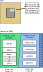
\includegraphics[scale=1]{img/proceso_en_memoria.pdf}
    \end{textblock}
\end{frame}

\begin{frame}{Ejecución de procesos}
    \small
    Los primeros sistemas eran \textbf{monotarea}.\\
    \textcolor{verdeuca}{Un \textbf{solo} proceso podia estar utilizando el procesador y acceder a los recursos del sistema.}\\
    \bigskip
    \pause
    Los programas se ejecutaban uno a uno en orden de llegada, como \emph{procesos batch}.\\ %y era característico de los primeros sistemas de computo
    \textcolor{gray}{Cada programa resolvía una tarea específica sobre distintos conjuntos de datos de entrada.}\\
    \begin{center}
        \includegraphics[scale=1.5]{img/round_robin-layer1.pdf}
    \end{center}
    \pause
    Las primeras computadoras hogareñas seguían este modelo y permitían ejecutar sólo una tarea por vez.\\
    No compartían recursos y sí los compartían los utilizaban cooperativamente entre procesos.\\
    \textcolor{naranjauca}{MS-DOS es un ejemplo de este sistema.}\\
    \bigskip
    Los sistemas más avanzados tenían la posibilidad de ejecutar múltiples procesos concurrentemente a pesar de tener un solo procesador.
    \pause
    \begin{center}
    \textcolor{naranjauca}{\textbf{Pero, ¿Cómo ejecutan múltiples procesos en un solo procesador?}}
    \end{center}
\end{frame}

\begin{frame}{Ejecución de múltiples procesos: \emph{Multitasking}}
    \begin{center}
    Para simular que ejecutamos \textbf{simultáneamente} varios procesos,\\ vamos a ejecutar por una fracción de tiempo cada uno, una y otra vez.
    \end{center}
    \begin{center}
        \includegraphics[scale=1.5]{img/round_robin-layer1.pdf}
    \end{center}
    \pause
    \textcolor{verdeuca}{Vamos a hacer esto tan rápido que el usuario \textbf{no va a percibir} que en realidad hay un solo proceso corriendo por unidad de tiempo.}
    Ejecutamos los procesos \textbf{concurrentemente}.\\
    \begin{center}
        \includegraphics[scale=1.5]{img/round_robin-layer2.pdf}
    \end{center}
    \pause
    \begin{center}
    \textcolor{naranjauca}{El tiempo del procesador es compartido por múltiples procesos en ejecución.}\\
    \vspace{0.2cm}
    \small
    El sistema operativo cuenta con un componente denominado \emph{scheduler}\\ o \textbf{planificador}, que decide cual será el próximo proceso en ser ejecutado.
    \end{center}
\end{frame}

\begin{frame}[fragile]{Estados de un proceso}
    \begin{textblock}{55}(7,15)
    \small
    Los procesos antes de comenzar a ser ejecutados o mientras son ejecutados pueden tomar múltiples \textbf{estados}.\\
    \end{textblock}
    \begin{textblock}{140}(5,30)
    \small
    \begin{itemize}
    \setlength\itemsep{0cm}
    \item<2->[-] \textbf{Nuevo}: Estado inicial, el proceso se está cargando\\ poco a poco en memoria y solicitando recursos.
    \item<3->[-] \textbf{Preparado}: El proceso puede ser ejecutado, pero el procesador aun no está disponible.
    \item<4->[-] \textbf{En Ejecución}: El proceso está siendo ejecutado actualmente. Existe un solo proceso en este estado.
    \item<5->[-] \textbf{Terminado}: Proceso terminado, no puede volver a correr. Aun existe en la medida que desalojen todos sus recursos.
    \end{itemize}
    \uncover<6->{Pasar de \textbf{En Ejecución} a \textbf{Preparado} es posible cuando se \emph{pausa} o \emph{desaloja} un proceso.}
    \begin{itemize}
    \setlength\itemsep{0cm}
    \item<7-> \textbf{En Espera}: El proceso queda en espera por un evento, será pasado a \emph{Preparado} cuando suceda el evento por el cual espera.
    \end{itemize}
    \begin{center}
     \uncover<8->{\textcolor{naranjauca}{\large \textbf{¿Cómo espera un proceso?}}}
    \end{center}
    \end{textblock}
    \begin{textblock}{100}(80,6) \only<2->{\includegraphics[scale=1.2]{img/estados-layer1.pdf}} \end{textblock} % nuevo
    \begin{textblock}{100}(80,6) \only<3->{\includegraphics[scale=1.2]{img/estados-layer2.pdf}} \end{textblock} % preparado
    \begin{textblock}{100}(80,6) \only<4->{\includegraphics[scale=1.2]{img/estados-layer3.pdf}} \end{textblock} % en ejecucion
    \begin{textblock}{100}(80,6) \only<5->{\includegraphics[scale=1.2]{img/estados-layer5.pdf}} \end{textblock} % terminado
    \begin{textblock}{100}(80,6) \only<6->{\includegraphics[scale=1.2]{img/estados-layer4.pdf}} \end{textblock} % - pause
%     \begin{textblock}{100}(80,6) \only<6->{\includegraphics[scale=1.2]{img/estados-layer6.pdf}} \end{textblock} % - dispatch
%     \begin{textblock}{100}(80,6) \only<7->{\includegraphics[scale=1.2]{img/estados-layer7.pdf}} \end{textblock} % - interrupcion
    \begin{textblock}{100}(80,6) \only<7->{\includegraphics[scale=1.2]{img/estados-layer8.pdf}} \end{textblock} % en espera
\end{frame}

% \begin{frame}[fragile]{Estados de un proceso}
%     \begin{itemize}
%     \item[-] \emph{New}$\rightarrow$\emph{Ready}: Disponible para ser ejecutado.
%     \item[-] \emph{Ready}$\rightarrow$\emph{Running}: Pasa a ser ejecutado.
%     \item[-] \emph{Running}$\rightarrow$\emph{Ready}: Desalojado del procesador.
%     \item[-] \emph{Running}$\rightarrow$\emph{Terminated}: Termina y libera recursos.
%     \item[-] \emph{Running}$\rightarrow$\emph{Waiting}: Pasa a esperar un evento.
%     \item[-] \emph{Waiting}$\rightarrow$\emph{Ready}: Sucede el evento por el que se esperaba y pasa a estar listo para continuar ejecutando.     
%     \end{itemize}
% \end{frame}

\begin{frame}{Colas de espera}
    \begin{textblock}{100}(10,12)
    \small
    Los procesos aguardan por su turno en colas de procesos.
    \end{textblock}
    \begin{textblock}{100}(20,20)
    \includegraphics[scale=1]{img/queues-layer1.pdf}
    \end{textblock}
    \begin{textblock}{100}(90,18) \only<1->{\includegraphics[scale=0.9]{img/estados-layer1.pdf}} \end{textblock} % nuevo
    \begin{textblock}{100}(90,18) \only<1->{\includegraphics[scale=0.9]{img/estados-layer2.pdf}} \end{textblock} % preparado
    \begin{textblock}{100}(90,18) \only<1->{\includegraphics[scale=0.9]{img/estados-layer3.pdf}} \end{textblock} % en ejecucion
    \begin{textblock}{100}(90,18) \only<1->{\includegraphics[scale=0.9]{img/estados-layer5.pdf}} \end{textblock} % terminado
    \begin{textblock}{100}(90,18) \only<1->{\includegraphics[scale=0.9]{img/estados-layer4.pdf}} \end{textblock} % - pause
    \begin{textblock}{140}(10,40)
    \small
    \uncover<2->{Una vez dentro de la CPU, los procesos pueden ser \emph{pausados}, \emph{desalojados} o \emph{terminados}.}\\
    \bigskip
    \uncover<3->{Si el proceso decide ser \emph{pausado}, el sistema se denomina \textbf{cooperativo}.}\\
    \medskip
    \uncover<4->{Si el proceso es \emph{desalojado} en cualquier momento por el sistema, se dice que el sistema tiene \textbf{desalojo} o es \textbf{apropiativo}.}\\
    \end{textblock}
\end{frame}

\begin{frame}{Colas de espera}
    \begin{textblock}{100}(10,12)
    \small
    Un proceso bloqueado por entrada/salida espera en una cola diferente.
    \end{textblock}
    \begin{textblock}{100}(20,20)
    \includegraphics[scale=1]{img/queues-layer2.pdf}
    \end{textblock}
    \begin{textblock}{100}(90,18) \only<1->{\includegraphics[scale=0.9]{img/estados-layer1.pdf}} \end{textblock} % nuevo
    \begin{textblock}{100}(90,18) \only<1->{\includegraphics[scale=0.9]{img/estados-layer2.pdf}} \end{textblock} % preparado
    \begin{textblock}{100}(90,18) \only<1->{\includegraphics[scale=0.9]{img/estados-layer3.pdf}} \end{textblock} % en ejecucion
    \begin{textblock}{100}(90,18) \only<1->{\includegraphics[scale=0.9]{img/estados-layer5.pdf}} \end{textblock} % terminado
    \begin{textblock}{100}(90,18) \only<1->{\includegraphics[scale=0.9]{img/estados-layer4.pdf}} \end{textblock} % - pause
    \begin{textblock}{100}(90,18) \only<1->{\includegraphics[scale=0.9]{img/estados-layer8.pdf}} \end{textblock} % en espera
    \begin{textblock}{140}(10,50)
    \small
    \uncover<2->{\textcolor{naranjauca}{No todos los eventos de entrada salida demorarán el mismo tiempo.}}\\ 
    \medskip
    \uncover<3->{Por lo tanto podemos crear \textbf{múltiples colas de espera} dependiendo de la razón del desalojo.}\\
    \medskip
    \uncover<4->{\textcolor{gray}{Existirán colas de espera por eventos como escribir en pantalla, o escribir un archivo,\\
    como también por leer entradas del teclado.}}
    \end{textblock}
\end{frame}

\begin{frame}{Colas de espera}
    \begin{textblock}{100}(10,12)
    \small
    Un proceso bloqueado por entrada/salida espera en una cola diferente.
    \end{textblock}
    \begin{textblock}{100}(20,20)
    \includegraphics[scale=1]{img/queues-layer3.pdf}
    \end{textblock}
    \begin{textblock}{100}(90,18) \only<1->{\includegraphics[scale=0.9]{img/estados-layer1.pdf}} \end{textblock} % nuevo
    \begin{textblock}{100}(90,18) \only<1->{\includegraphics[scale=0.9]{img/estados-layer2.pdf}} \end{textblock} % preparado
    \begin{textblock}{100}(90,18) \only<1->{\includegraphics[scale=0.9]{img/estados-layer3.pdf}} \end{textblock} % en ejecucion
    \begin{textblock}{100}(90,18) \only<1->{\includegraphics[scale=0.9]{img/estados-layer5.pdf}} \end{textblock} % terminado
    \begin{textblock}{100}(90,18) \only<1->{\includegraphics[scale=0.9]{img/estados-layer4.pdf}} \end{textblock} % - pause
    \begin{textblock}{100}(90,18) \only<1->{\includegraphics[scale=0.9]{img/estados-layer8.pdf}} \end{textblock} % en espera
    \begin{textblock}{140}(10,70)
    \small
    Las múltiples colas de espera, permiten \textbf{ordenar los tiempos de espera} entre los distintos procesos.\\
    Reduciendo el tiempo máximo que un proceso debe esperar en caso de ser encolado.
    \end{textblock}
\end{frame}

\begin{frame}{Bloque de Control de Proceso (PCB - \emph{Process Control Block})}
    \normalsize
    El \textbf{PCB} es la estructura de datos dentro del Sistema Operativo\\ que almacena toda la \textcolor{verdeuca}{\textbf{información de un proceso}}.
    \medskip
    \pause
    \small
    \begin{itemize}\setlength\itemsep{0.2cm}
    \item[-] Identificador del proceso (\texttt{PID})
    \item[-] Estado del proceso en el CPU\\
    \hspace{0.5cm}\textcolor{gray}{Registros (\emph{Program Counter}, Flags, Pila, etc.)}
    \item[-] Información de planificación\\
    \hspace{0.5cm}\textcolor{gray}{Estadísticas, Prioridades, Tipos de procesos, etc.}
    \item[-] Información para la gestión de memoria del proceso\\
    \hspace{0.5cm}\textcolor{gray}{Memoria asignada, Memoria libre, etc.}
    \item[-] Información sobre la E/S del proceso\\
    \hspace{0.5cm}\textcolor{gray}{Archivos abiertos, \emph{Sockets} asignados, \emph{Buffers}, etc.}
    \end{itemize}
    \begin{textblock}{60}(95,25)
    \uncover<3->{
    \begin{tcolorbox}[size=small,width=\textwidth,sharp corners,title={}]
     \footnotesize
     Los \texttt{PCB} se suelen administrar como \textbf{listas\\ enlazadas}, modelando así la funcionalidad\\ de una cola de procesos.
     \begin{center}
     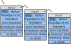
\includegraphics[scale=0.75]{img/pcb_lista.pdf}
     \end{center}
     \vspace{0.1cm}
    \end{tcolorbox}
    }
    \end{textblock}
\end{frame}

\begin{frame}[t]{Cambio de contexto (\emph{context switch})}
    Cuando se debe intercambiar al proceso que se encuentra corriendo por otro,\\ se da un cambio de contexto.\\
    \bigskip
    Este procedimiento se puede dar en bajo tres condiciones:
    \begin{itemize}
    \item Se produce una \textbf{excepción} de protección.
    \item Se produce una \textbf{interrupción} de E/S.
    \item Se \textbf{termina} el tiempo (\emph{quantum}) que el proceso tenia asignado.% que está ejecutando actualmente.
    \end{itemize}
    \pause
    \bigskip
    Un cambio de contexto implica una operatoria compleja, en la cual se captura una \textbf{\textcolor{naranjauca}{foto}} del\\
    contexto de ejecución actual y se lo intercambia por otro contexto de ejecución diferente.\\
    \bigskip
    \begin{center}
    \textcolor{naranjauca}{\textbf{¿Qué tareas implica un cambio de contexto?}}
    \end{center}
\end{frame}

\begin{frame}[t]{Cambio de contexto (\emph{context switch})}
    Procedimiento para el cambio de contexto entre \texttt{PCB$_\text{0}$} y \texttt{PCB$_\text{1}$}:\\
    \vspace{0.2cm}
    \begin{enumerate}
    \small
    \setlength\itemsep{0.1cm}
    \item<3-> Guardar el contexto de ejecución (el estado del procesador) en el \texttt{PCB$_\text{0}$}.
    \item<4-> Actualizar el estado del \texttt{PCB$_\text{0}$} para indicar que no está más en ejecución.
    \item<5-> Restaurar el contexto de ejecución del \texttt{PCB$_\text{1}$}.
    \item<6-> Actualizar las estructuras de datos para la administración de memoria del \texttt{PCB$_\text{1}$}.
    \item<7-> Actualizar el estado del \texttt{PCB$_\text{1}$} para indicar que esta siendo ejecutado.
    \item<8-> Retorna el control al proceso.
    \end{enumerate}
    \begin{textblock}{100}(15,53) \only<1->{\includegraphics[scale=1.6]{img/intercambio_de_tareas-layer1.pdf}} \end{textblock} % 
    \begin{textblock}{100}(15,53) \only<2->{\includegraphics[scale=1.6]{img/intercambio_de_tareas-layer2.pdf}} \end{textblock} % 
    \begin{textblock}{100}(15,53) \only<3->{\includegraphics[scale=1.6]{img/intercambio_de_tareas-layer3.pdf}} \end{textblock} % 
    \begin{textblock}{100}(15,53) \only<5->{\includegraphics[scale=1.6]{img/intercambio_de_tareas-layer4.pdf}} \end{textblock} % 
    \begin{textblock}{100}(15,53) \only<8->{\includegraphics[scale=1.6]{img/intercambio_de_tareas-layer5.pdf}} \end{textblock} % 
    \begin{textblock}{100}(15,53) \only<9->{\includegraphics[scale=1.6]{img/intercambio_de_tareas-layer6.pdf}} \end{textblock} % latencia
    \begin{textblock}{60}(95,55)
    \uncover<9->{
    \begin{tcolorbox}[size=small,width=\textwidth,sharp corners,title={}]
    \scriptsize
    Cada cambio de contexto demora tiempo (\emph{latencia}).
    El procesador dispone de \textbf{mecanismos en hardware} para reducir este tiempo.\\
    Aun así, actualizar las estructuras de administración de memoria es muy costoso.
    \end{tcolorbox}
    }
    \end{textblock}
\end{frame}

\begin{frame}{Creación de un nuevo proceso}
    \begin{textblock}{100}(10,12)
    \small
    Para crear un nuevo proceso se debe:
    \begin{enumerate}
    \item<1-> Asignar un identificador único al nuevo proceso (\texttt{PID}).
    \item<2-> Reservar un espacio en memoria para el nuevo proceso.
    \item<3-> Inicializar un nuevo PCB.
    \item<4-> Enlazar el nuevo PCB en las estructuras de datos del sistema.
    \end{enumerate}
    \end{textblock}
    \begin{textblock}{80}(10,45)
    \small
    \uncover<5->{Los nuevos procesos son creados por otros procesos,\\ utilizando la \emph{syscall} \texttt{fork}.}\\
    \medskip
    \uncover<5->{Al proceso creador se lo llama \texttt{padre} (\emph{parent}),\\ mientras que al proceso \texttt{hijo} (\emph{child}).}\\
    \medskip
    \uncover<6->{Un proceso puede tener múltiples procesos hijos,\\ pero todos los procesos tienen un sólo proceso padre.}\\
    \medskip
    \uncover<6->{Este comportamiento configura un \textbf{árbol de procesos}.}
    \end{textblock}
    \begin{textblock}{100}(100,8) \includegraphics[scale=0.5]{img/process_tree-layer1.pdf} \end{textblock}
\end{frame}

\begin{frame}{Creación de un nuevo proceso: En \texttt{UNIX}}
    \begin{textblock}{120}(10,12)
    \small
    Para crear un nuevo proceso se utilizan dos llamados al sistema:
    \begin{itemize}
     \item[-] \textcolor{naranjauca}{\texttt{fork()}}: Crea un nuevo proceso hijo con la misma memoria del proceso padre.
     \item[-] \textcolor{naranjauca}{\texttt{exec()}}: Remplaza la memoria del proceso por la de un nuevo programa.
    \end{itemize}
    \end{textblock}
    \begin{textblock}{100}(10,35) \only<2->{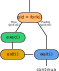
\includegraphics[scale=0.6]{img/fork_exec.pdf}} \end{textblock}
    \begin{textblock}{90}(55,35)
    \small
    \uncover<3->{\textcolor{gray}{
    Al ser creado un nuevo proceso, este \textbf{copia todo el estado del proceso padre}.
    Se diferenciarán en el valor de retorno del \texttt{fork}.}}\\
    \bigskip
    \uncover<3->{\textcolor{gray}{
    Esto permite modificar el comportamiento del proceso y llamar al servicio \texttt{exec},
    que \textbf{remplaza toda la memoria del proceso original} por la de un nuevo programa.}}\\
    \bigskip
    \uncover<3->{\textcolor{gray}{
    El nuevo proceso, \textbf{con un código diferente}, es ejecutado hasta que decide terminar llamando a \texttt{exit}.}}\\
    \bigskip
    \uncover<3->{\textcolor{gray}{
    El proceso padre puede llamar a \texttt{wait} para esperar la finalización del proceso hijo.}}\\
    \end{textblock}
\end{frame}

\begin{frame}[t]{Terminación de un proceso}
    La terminación de un proceso se puede dar en las siguientes situaciones:
    \begin{itemize}
    \item[-] El proceso \textcolor{naranjauca}{\textbf{decide terminar}} llamando a la \emph{syscall} \texttt{exit}.
    \item[-] El proceso \textcolor{naranjauca}{\textbf{genera un error}} y el Sistema Operativo lo termina.
    \item[-] El padre decide \textcolor{naranjauca}{\textbf{terminar al proceso hijo}} (\texttt{abort}).
    \item[-] \textcolor{naranjauca}{\textbf{El padre termina}} y por lo tanto los hijos también (terminación en cascada).
    \end{itemize}
    \medskip
    \pause
    \begin{tcolorbox}[size=small,width=0.7\textwidth,sharp corners,title={}]
    \small
    \color{verdeuca}
    Cuando un proceso termina el sistema debe \textbf{liberar sus recursos}:
    \begin{itemize} \color{verdeuca}
    \setlength\itemsep{0cm}
        \item[\textcolor{verdeuca}{-}] Liberar la memoria asignada.
        \item[\textcolor{verdeuca}{-}] Liberar descriptores de archivos abiertos.
        \item[\textcolor{verdeuca}{-}] Liberar los \emph{buffers} de entrada/salida en uso.
    \end{itemize}
    \end{tcolorbox}
    \medskip
    \pause
    El proceso padre, puede \textcolor{verdeuca}{\textbf{esperar por la terminación}} del proceso hijo llamando a \texttt{wait}.\\
    \medskip
    El servicio \emph{wait} retorna al padre el \textcolor{verdeuca}{\textbf{estado de terminación}} del proceso hijo.
\end{frame}

\begin{frame}[t]{\emph{Threads} (Hilos)}
    \small
    \uncover<1->{Crear nuevos procesos, implica la costosa tarea de administrar la memoria para estos nuevos procesos.\\
    Para reducir el \textbf{costo de crear nuevos contextos de ejecución}, existen los \emph{threads} o hilos de ejecución.}\\
    \bigskip
    \uncover<2->{Los \emph{threads} son \textbf{nuevos contextos de ejecución}, similares a un nuevo proceso, pero que comparten recursos con el proceso padre.
    \textcolor{verdeuca}{Tienen el \textbf{mismo mapa de memoria} para código y datos que el padre.}}\\    
    \begin{textblock}{70}(10,40) \only<3->{Single-Thread} \end{textblock}
    \begin{textblock}{70}(10,45) \only<3->{\includegraphics[scale=1]{img/singlethread_multithread-layer1.pdf}} \end{textblock}
    \begin{textblock}{70}(10,45) \only<4->{\includegraphics[scale=1]{img/singlethread_multithread-layer2.pdf}} \end{textblock}
    \begin{textblock}{70}(80,40) \only<5->{Multi-Thread} \end{textblock}
    \begin{textblock}{70}(80,45) \only<5->{\includegraphics[scale=1]{img/singlethread_multithread-layer1.pdf}} \end{textblock}
    \begin{textblock}{70}(80,45) \only<5->{\includegraphics[scale=1]{img/singlethread_multithread-layer2.pdf}} \end{textblock}
    \begin{textblock}{70}(80,45) \only<6->{\includegraphics[scale=1]{img/singlethread_multithread-layer3.pdf}} \end{textblock}
    \begin{textblock}{70}(80,45) \only<7->{\includegraphics[scale=1]{img/singlethread_multithread-layer4.pdf}} \end{textblock}
\end{frame}

\begin{frame}[t]{\emph{Threads} (Hilos): Ejemplo}
    \begin{textblock}{50}(5,15)
    \small
    \uncover<1->{Un proceso hace tres \emph{requests} a un servicio externo, quedando bloqueado en cada llamado.\\}
    \medskip
    \uncover<13->{Si utilizamos \emph{threads} en cada llamado, el tiempo bloqueado es aprovechado otro \emph{thread}.\\}
    \medskip
    \uncover<14->{\textcolor{verdeuca}{Si bien se utiliza un solo procesador, esté queda bloqueado durante menos tiempo.}\\}
    \bigskip
    \uncover<15->{
    \begin{tcolorbox}[size=small,width=\textwidth,sharp corners,title={}]
    \scriptsize
    Utilizar \emph{threads} mejora la capacidad de\\
    respuesta de los procesos interactivos,\\
    mejorado el uso de los recursos del\\
    procesador y reduciendo la cantidad de\\
    memoria utilizada.
    \end{tcolorbox}
    }
    \end{textblock}
    \begin{textblock}{70}(60,15) \only<10->{\includegraphics[scale=1.3]{img/threads-layer10.pdf}} \end{textblock} % bloqueados todos    (ultimo)
    \begin{textblock}{70}(60,15) \only<7->{ \includegraphics[scale=1.3]{img/threads-layer7.pdf}}  \end{textblock} % multi th0 bloqueado (ultimo)
    \begin{textblock}{70}(60,15) \only<9->{ \includegraphics[scale=1.3]{img/threads-layer9.pdf}}  \end{textblock} % multi th2           (ultimo)
    \begin{textblock}{70}(60,15) \only<8->{ \includegraphics[scale=1.3]{img/threads-layer8.pdf}}  \end{textblock} % multi th1           (ultimo)
    \begin{textblock}{70}(60,15) \only<14->{\includegraphics[scale=1.3]{img/threads-layer14.pdf}} \end{textblock} % diferencia
    \begin{textblock}{70}(60,15) \only<13->{\includegraphics[scale=1.3]{img/threads-layer13.pdf}} \end{textblock} % multi th0 wait
    \begin{textblock}{70}(60,15) \only<12->{\includegraphics[scale=1.3]{img/threads-layer12.pdf}} \end{textblock} % multi th0, th1 y th2 join
    \begin{textblock}{70}(60,15) \only<11->{\includegraphics[scale=1.3]{img/threads-layer11.pdf}} \end{textblock} % multi th0 response
    \begin{textblock}{70}(60,15) \only<6->{ \includegraphics[scale=1.3]{img/threads-layer6.pdf}}  \end{textblock} % multi th0 paso new thread
    \begin{textblock}{70}(60,15) \only<5->{ \includegraphics[scale=1.3]{img/threads-layer5.pdf}}  \end{textblock} % multi th0 paso 0
    \begin{textblock}{70}(60,15) \only<4->{ \includegraphics[scale=1.3]{img/threads-layer4.pdf}}  \end{textblock} % single paso n resto
    \begin{textblock}{70}(60,15) \only<3->{ \includegraphics[scale=1.3]{img/threads-layer3.pdf}}  \end{textblock} % single paso 1 proceso
    \begin{textblock}{70}(60,15) \only<2->{ \includegraphics[scale=1.3]{img/threads-layer2.pdf}}  \end{textblock} % single paso 1 bloqueado
    \begin{textblock}{70}(60,15) \only<1->{ \includegraphics[scale=1.3]{img/threads-layer1.pdf}}  \end{textblock} % single paso 1
\end{frame}

\begin{frame}[t]{Comunicación entre procesos}
    \small
    Los procesos cooperativos necesitan comunicarse entre sí.\\
    Dos formas de IPC (\emph{Inter-process communication})
    \begin{textblock}{65}(10,20)
    \begin{center}
    \includegraphics[scale=0.6]{img/ipc-layer1.pdf}\\
    \textbf{Memoria compartida}\\
    \vspace{0.2cm} \small
    Un área de memoria compartida entre\\ dos o más procesos a nivel de usuario.
    \end{center}
    \end{textblock}
    \begin{textblock}{65}(85,20)
    \begin{center}
    \includegraphics[scale=0.6]{img/ipc-layer2.pdf}\\
    \textbf{Pasaje de Mensajes}\\
    \vspace{0.2cm} \small
    El Sistema Operativo proporciona un\\ mecanismo para enviar y recibir\\ mensajes entre procesos.
    \end{center}
    \end{textblock}
\end{frame}

\begin{frame}[t,fragile]{Comandos útiles en Linux}
    \begin{textblock}{90}(10,13)
    \small
    \textcolor{naranjauca}{\textbf{\texttt{ps}}}\\
    Muestra el estado de todos los procesos del sistema.\\
    \textcolor{gray}{Ejemplo:} \verb|$| \texttt{ps -aux} {\scriptsize \keys{\return}}\\
    \vspace{0.3cm}
    \textcolor{naranjauca}{\textbf{\texttt{top}}} o \textcolor{naranjauca}{\textbf{\texttt{htop}}}\\
    Muestra el consumo de CPU y memoria de cada proceso.\\
    \textcolor{gray}{Ejemplo:} \verb|$| \texttt{top} {\scriptsize \keys{\return}}\\
    \vspace{0.3cm}
    \textcolor{naranjauca}{\textbf{\texttt{pstree}}}\\
    Muestra el árbol de procesos de todo el sistema.\\
    \textcolor{gray}{Ejemplo:} \verb|$| \texttt{pstree -p} {\scriptsize \keys{\return}}\\
    \vspace{0.3cm}
    \textcolor{naranjauca}{\textbf{\texttt{kill}}}\\
    Envia un señal al proceso indicado por su \texttt{PID}.\\ Por defecto, envía la señal de terminación.\\
    \textcolor{gray}{Ejemplo:} \verb|$| \texttt{kill 1245} {\scriptsize \keys{\return}}\\
    \vspace{0.3cm}
    \footnotesize
    \textcolor{gray}{Para más información consultar los manuales\\ con el comando \texttt{man}}
    \end{textblock}
    \begin{textblock}{90}(92,5)
    \includegraphics[width=6.5cm]{img/ps.png}\\ \vspace{0.2cm}
    \includegraphics[width=6.5cm]{img/top.png}\\ \vspace{0.2cm}
    \includegraphics[width=6.5cm]{img/pstree.png}
    \end{textblock}
\end{frame}

\begin{frame}[fragile]
    \frametitle{Bibliografía}
    \begin{itemize}
        \setlength\itemsep{0.5cm}
        \item[-] \small Silberschatz, ``Fundamentos de Sistemas Operativos'', 7ma Edición, 2006.\\
        \begin{itemize}
            \item \textbf{Capítulo 3 - Procesos}, páginas 73-86
            \item \textbf{Capítulo 4 - Hebras}, páginas 113-115
        \end{itemize}
        \item[-] \small Stallings, ``Operating Systems: Internals and Design Principles'', 9th Edition, 2018.\\
        \begin{itemize}
            \item \textbf{Chapter 3 - Process Description and Control}, páginas 130-163
            \item \textbf{Chapter 4 - Threads}, páginas 177-183
        \end{itemize}
    \end{itemize}
\end{frame}

\begin{frame}[fragile]{Ejercicios}
    Con lo visto, ya pueden resolver todos los ejercicios de la Guía de Procesos.
\end{frame}

\begin{frame}[plain]
    \begin{center}
    \vspace{2cm}
    \huge ¡Gracias!\\
    \vspace{2cm}
%     \normalsize Recuerden leer los comentarios adjuntos\\ en cada clase por aclaraciones.
    \end{center}
\end{frame}

\end{document}

